% Source for fig_4_8_wireframes.pdf. Build: pdflatex fig_4_8_wireframes.tex
\documentclass[tikz,border=2pt]{standalone}
\usetikzlibrary{shapes.geometric}
\renewcommand{\familydefault}{\sfdefault}
\newcommand{\sw}{5.1}\newcommand{\sh}{7.4}
\newcommand{\screen}[2]{% number, title
  \draw[rounded corners=4pt,thick] (0,0) rectangle (\sw,-\sh);
  \fill[black!12,rounded corners=4pt] (.03,-.03) rectangle (\sw-.03,-.62);
  \node[anchor=west,font=\scriptsize\bfseries] at (.15,-.32) {#2};
  \node[anchor=south west,font=\scriptsize\bfseries,inner sep=0pt] at (0,.08) {Wireframe #1};}
\newcommand{\lbl}[3]{\node[anchor=north west,inner sep=0pt,font=\tiny,text width=#3 cm,align=left] at (.2,#1) {#2};}
\newcommand{\fld}[4]{% x, y, w, text
  \draw[rounded corners=1pt] (#1,#2) rectangle ++(#3,-.42);
  \node[anchor=west,font=\tiny,inner sep=2pt] at (#1,#2-.21) {#4};}
\newcommand{\btn}[5][black!70]{% fill; x, y, w, text
  \draw[rounded corners=2pt,fill=#1] (#2,#3) rectangle ++(#4,-.46);
  \node[font=\tiny\bfseries,text=white] at (#2+#4/2,#3-.23) {#5};}
\newcommand{\gbtn}[4]{% disabled or secondary; x, y, w, text
  \draw[rounded corners=2pt,fill=black!10] (#1,#2) rectangle ++(#3,-.46);
  \node[font=\tiny\bfseries] at (#1+#3/2,#2-.23) {#4};}
\newcommand{\mk}[3]{\node[circle,fill=black,text=white,font=\tiny\bfseries,inner sep=.6pt,minimum size=3.2mm] at (#1,#2) {#3};}
\tikzset{
  gGood/.style={circle,draw,fill=black!10,minimum size=2.4mm,inner sep=0pt},
  gMinor/.style={regular polygon,regular polygon sides=3,draw,fill=black!10,minimum size=3mm,inner sep=0pt},
  gMajor/.style={regular polygon,regular polygon sides=4,draw,fill=black!45,minimum size=3.2mm,inner sep=0pt},
  gMixed/.style={diamond,draw,fill=black!25,minimum size=3mm,inner sep=0pt},
  gNone/.style={circle,draw,dashed,minimum size=2.4mm,inner sep=0pt},
  chip/.style={draw,rounded corners=3pt,font=\tiny,inner sep=2.5pt}}
\newcommand{\grade}[4]{\node[#1] at (#2,#3) {}; \node[anchor=west,font=\tiny\bfseries,inner sep=0pt] at (#2+.2,#3) {#4};}
\begin{document}
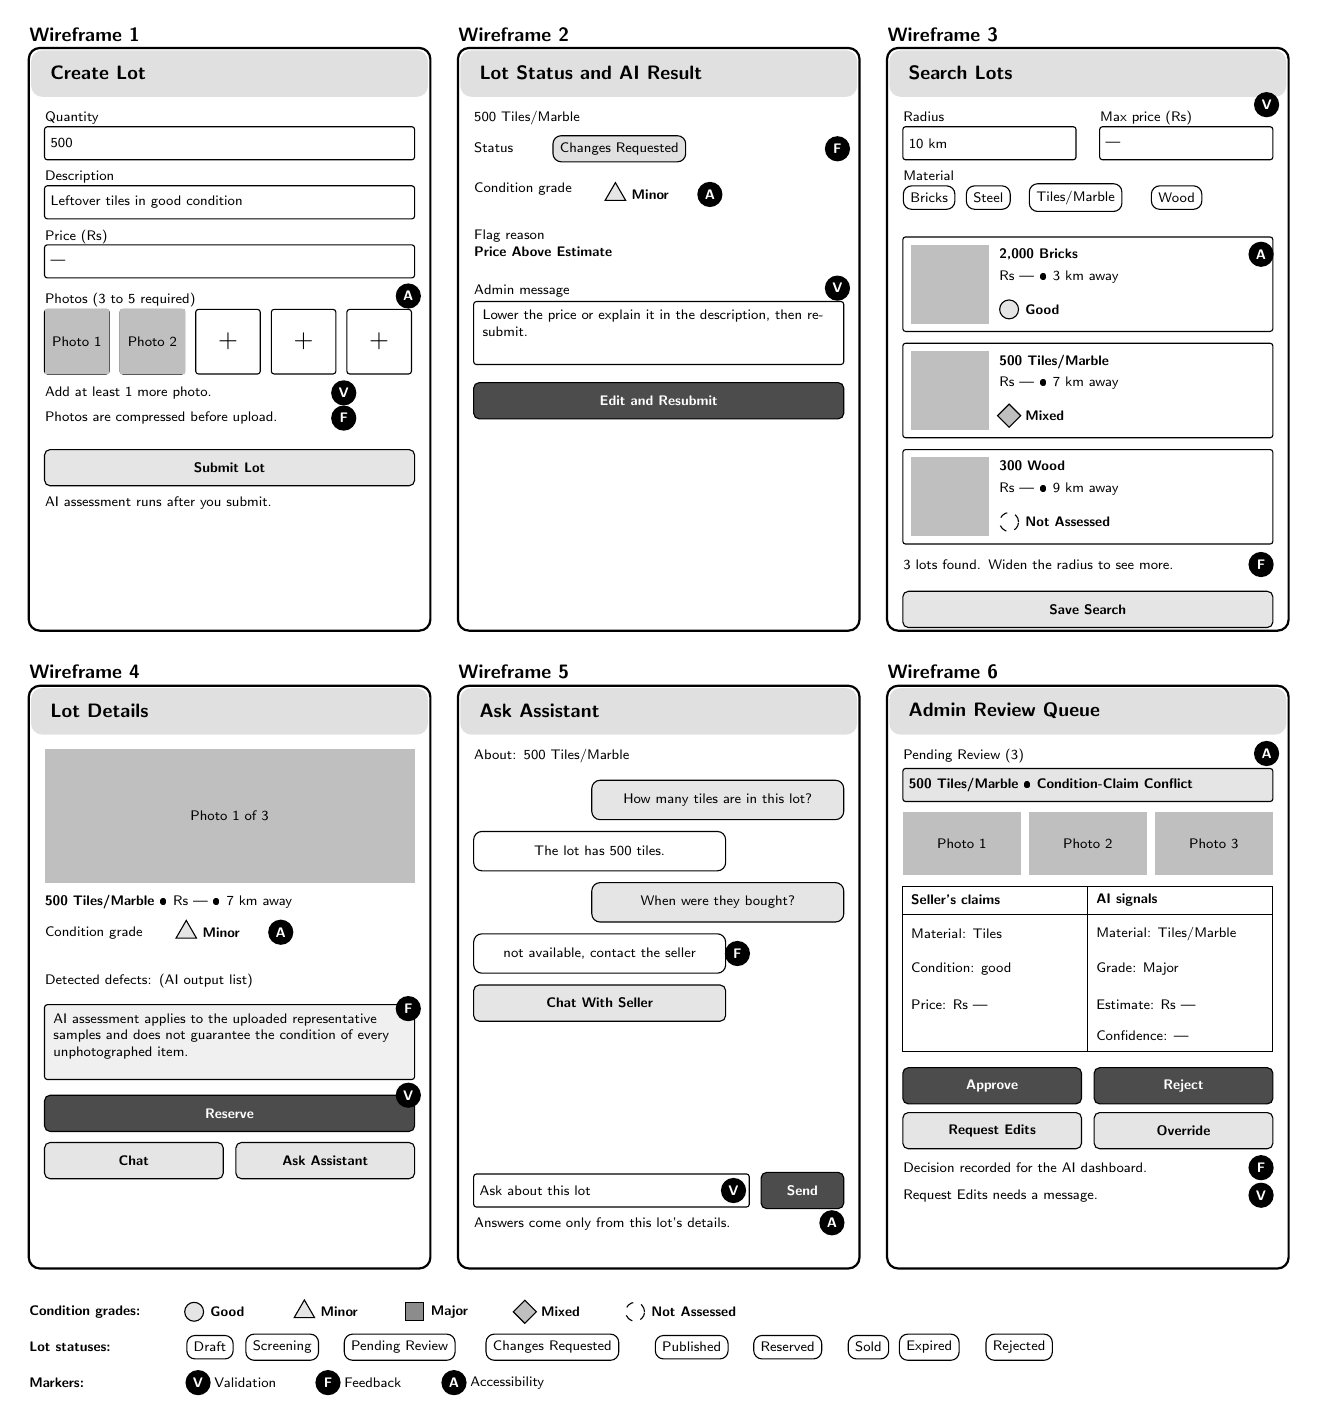
\begin{tikzpicture}
% 1 Create Lot
\begin{scope}
\screen{1}{Create Lot}
\lbl{-.8}{Quantity}{4}\fld{.2}{-1.0}{4.7}{500}
\lbl{-1.55}{Description}{4}\fld{.2}{-1.75}{4.7}{Leftover tiles in good condition}
\lbl{-2.3}{Price (Rs)}{4}\fld{.2}{-2.5}{4.7}{---}
\lbl{-3.1}{Photos (3 to 5 required)}{4}
\foreach \i in {0,1,2,3,4}{\draw[rounded corners=1pt] (.2+\i*.96,-3.32) rectangle ++(.82,-.82);}
\foreach \i in {0,1}{\fill[black!25] (.2+\i*.96,-3.32) rectangle ++(.82,-.82);\node[font=\tiny] at (.61+\i*.96,-3.73) {Photo \the\numexpr\i+1\relax};}
\foreach \i in {2,3,4}{\node[font=\small] at (.61+\i*.96,-3.73) {+};}
\lbl{-4.3}{Add at least 1 more photo.}{4.6}
\lbl{-4.62}{Photos are compressed before upload.}{4.6}
\gbtn{.2}{-5.1}{4.7}{Submit Lot}
\lbl{-5.7}{AI assessment runs after you submit.}{4.6}
\mk{4.82}{-3.15}{A}\mk{4.0}{-4.38}{V}\mk{4.0}{-4.7}{F}
\end{scope}
% 2 Lot status and AI result
\begin{scope}[shift={(5.45,0)}]
\screen{2}{Lot Status and AI Result}
\lbl{-.8}{500 Tiles/Marble}{4.6}
\lbl{-1.2}{Status}{1.5}\node[chip,fill=black!12,anchor=west] at (1.2,-1.28) {Changes Requested};
\lbl{-1.7}{Condition grade}{1.5}\grade{gMinor}{2.0}{-1.86}{Minor}
\lbl{-2.3}{Flag reason}{4.6}
\node[anchor=north west,font=\tiny\bfseries,inner sep=0pt] at (.2,-2.52) {Price Above Estimate};
\lbl{-3.0}{Admin message}{4.6}
\draw[rounded corners=1pt] (.2,-3.22) rectangle ++(4.7,-.8);
\node[anchor=north west,font=\tiny,text width=4.45cm,inner sep=3pt] at (.2,-3.22) {Lower the price or explain it in the description, then resubmit.};
\btn{.2}{-4.25}{4.7}{Edit and Resubmit}
\mk{4.82}{-1.28}{F}\mk{3.2}{-1.86}{A}\mk{4.82}{-3.05}{V}
\end{scope}
% 3 Search results
\begin{scope}[shift={(10.9,0)}]
\screen{3}{Search Lots}
\lbl{-.8}{Radius}{1.4}\fld{.2}{-1.0}{2.2}{10 km}
\node[anchor=north west,inner sep=0pt,font=\tiny] at (2.7,-.8) {Max price (Rs)};\fld{2.7}{-1.0}{2.2}{---}
\lbl{-1.55}{Material}{4}
\foreach \t/\x in {Bricks/.2,Steel/1.0,{Tiles/Marble}/1.8,Wood/3.35}{\node[chip,anchor=west,fill=white] at (\x,-1.9) {\t};}
\foreach \y/\t/\s/\g/\gn in {-2.4/{2,000 Bricks}/3 km away/gGood/Good,-3.75/{500 Tiles/Marble}/7 km away/gMixed/Mixed,-5.1/300 Wood/9 km away/gNone/Not Assessed}{
  \draw[rounded corners=1pt] (.2,\y) rectangle ++(4.7,-1.2);
  \fill[black!25] (.3,\y-.1) rectangle ++(1,-1);
  \node[anchor=north west,font=\tiny\bfseries,inner sep=0pt] at (1.42,\y-.14) {\t};
  \node[anchor=north west,font=\tiny,inner sep=0pt] at (1.42,\y-.42) {Rs --- \textbullet{} \s};
  \grade{\g}{1.55}{\y-.92}{\gn}
}
\lbl{-6.5}{3 lots found. Widen the radius to see more.}{4.6}
\gbtn{.2}{-6.9}{4.7}{Save Search}
\mk{4.82}{-.72}{V}\mk{4.75}{-6.56}{F}\mk{4.75}{-2.62}{A}
\end{scope}
% 4 Lot details
\begin{scope}[shift={(0,-8.1)}]
\screen{4}{Lot Details}
\fill[black!25] (.2,-.8) rectangle ++(4.7,-1.7);
\node[font=\tiny] at (2.55,-1.65) {Photo 1 of 3};
\lbl{-2.65}{\textbf{500 Tiles/Marble} \textbullet{} Rs --- \textbullet{} 7 km away}{4.6}
\lbl{-3.05}{Condition grade}{1.5}\grade{gMinor}{2.0}{-3.13}{Minor}
\lbl{-3.65}{Detected defects: (AI output list)}{4.6}
\draw[rounded corners=1pt,fill=black!6] (.2,-4.05) rectangle ++(4.7,-.95);
\node[anchor=north west,font=\tiny,text width=4.45cm,inner sep=3pt] at (.2,-4.05) {AI assessment applies to the uploaded representative samples and does not guarantee the condition of every unphotographed item.};
\btn{.2}{-5.2}{4.7}{Reserve}
\gbtn{.2}{-5.8}{2.27}{Chat}\gbtn{2.63}{-5.8}{2.27}{Ask Assistant}
\mk{3.2}{-3.13}{A}\mk{4.82}{-4.1}{F}\mk{4.82}{-5.2}{V}
\end{scope}
% 5 Chat with assistant
\begin{scope}[shift={(5.45,-8.1)}]
\screen{5}{Ask Assistant}
\lbl{-.8}{About: 500 Tiles/Marble}{4.6}
\draw[rounded corners=3pt,fill=black!10] (1.7,-1.2) rectangle ++(3.2,-.5);
\node[font=\tiny] at (3.3,-1.45) {How many tiles are in this lot?};
\draw[rounded corners=3pt] (.2,-1.85) rectangle ++(3.2,-.5);
\node[font=\tiny] at (1.8,-2.1) {The lot has 500 tiles.};
\draw[rounded corners=3pt,fill=black!10] (1.7,-2.5) rectangle ++(3.2,-.5);
\node[font=\tiny] at (3.3,-2.75) {When were they bought?};
\draw[rounded corners=3pt] (.2,-3.15) rectangle ++(3.2,-.5);
\node[font=\tiny] at (1.8,-3.4) {not available, contact the seller};
\gbtn{.2}{-3.8}{3.2}{Chat With Seller}
\fld{.2}{-6.2}{3.5}{Ask about this lot}
\btn{3.85}{-6.18}{1.05}{Send}
\lbl{-6.75}{Answers come only from this lot's details.}{4.6}
\mk{3.55}{-3.4}{F}\mk{4.75}{-6.82}{A}\mk{3.5}{-6.41}{V}
\end{scope}
% 6 Admin review queue
\begin{scope}[shift={(10.9,-8.1)}]
\screen{6}{Admin Review Queue}
\lbl{-.8}{Pending Review (3)}{2.5}
\draw[rounded corners=1pt,fill=black!10] (.2,-1.05) rectangle ++(4.7,-.42);
\node[anchor=west,font=\tiny\bfseries,inner sep=2pt] at (.2,-1.26) {500 Tiles/Marble \textbullet{} Condition-Claim Conflict};
\foreach \i in {0,1,2}{\fill[black!25] (.2+\i*1.6,-1.6) rectangle ++(1.5,-.8);}
\node[font=\tiny,inner sep=0pt] at (.95,-2.0) {Photo 1};\node[font=\tiny,inner sep=0pt] at (2.55,-2.0) {Photo 2};\node[font=\tiny,inner sep=0pt] at (4.15,-2.0) {Photo 3};
\draw (.2,-2.55) rectangle ++(4.7,-2.1);\draw (2.55,-2.55) -- ++(0,-2.1);\draw (.2,-2.9) -- ++(4.7,0);
\node[anchor=west,font=\tiny\bfseries,inner sep=0pt] at (.3,-2.72) {Seller's claims};
\node[anchor=west,font=\tiny\bfseries,inner sep=0pt] at (2.65,-2.72) {AI signals};
\foreach \y/\l/\r in {-3.15/Material: Tiles/{Material: Tiles/Marble},-3.6/Condition: good/Grade: Major,-4.05/Price: Rs ---/Estimate: Rs ---}{
  \node[anchor=west,font=\tiny,inner sep=0pt] at (.3,\y) {\l};
  \node[anchor=west,font=\tiny,inner sep=0pt] at (2.65,\y) {\r};}
\node[anchor=west,font=\tiny,inner sep=0pt] at (2.65,-4.45) {Confidence: ---};
\btn{.2}{-4.85}{2.27}{Approve}\btn{2.63}{-4.85}{2.27}{Reject}
\gbtn{.2}{-5.42}{2.27}{Request Edits}\gbtn{2.63}{-5.42}{2.27}{Override}
\lbl{-6.05}{Decision recorded for the AI dashboard.}{4.3}
\lbl{-6.4}{Request Edits needs a message.}{4.3}
\mk{4.82}{-.86}{A}\mk{4.75}{-6.12}{F}\mk{4.75}{-6.47}{V}
\end{scope}
% Legend
\node[anchor=west,font=\tiny\bfseries,inner sep=0pt] at (0,-16.05) {Condition grades:};
\grade{gGood}{2.1}{-16.05}{Good}\grade{gMinor}{3.5}{-16.05}{Minor}\grade{gMajor}{4.9}{-16.05}{Major}\grade{gMixed}{6.3}{-16.05}{Mixed}\grade{gNone}{7.7}{-16.05}{Not Assessed}
\node[anchor=west,font=\tiny\bfseries,inner sep=0pt] at (0,-16.5) {Lot statuses:};
\foreach \t/\x in {Draft/2.0,Screening/2.75,Pending Review/4.0,Changes Requested/5.8,Published/7.95,Reserved/9.2,Sold/10.4,Expired/11.05,Rejected/12.15}{\node[chip,anchor=west] at (\x,-16.5) {\t};}
\node[anchor=west,font=\tiny\bfseries,inner sep=0pt] at (0,-16.95) {Markers:};
\mk{2.15}{-16.95}{V}\node[anchor=west,font=\tiny,inner sep=0pt] at (2.35,-16.95) {Validation};
\mk{3.8}{-16.95}{F}\node[anchor=west,font=\tiny,inner sep=0pt] at (4.0,-16.95) {Feedback};
\mk{5.4}{-16.95}{A}\node[anchor=west,font=\tiny,inner sep=0pt] at (5.6,-16.95) {Accessibility};
\end{tikzpicture}
\end{document}
